% diagrams/lineas-cuadrado.tex -- un cuadrado y dos trazos sueltos,
% deliberadamente SIN forma cerrada, para la actividad "Completa": la
% niña o el niño los convierte en su propio dibujo (una casa, un
% regalo, una caja, una mesa, un robot... lo que se le ocurra, o lo que
% pida el enunciado de ese día).
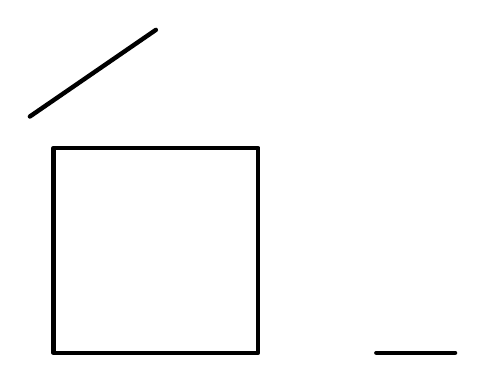
\begin{tikzpicture}[line width=1.6pt, line cap=round, line join=round]
  \draw (-1.3,-2.4) rectangle (1.3,0.2);
  \draw (-1.6,0.6) -- (0,1.7);
  \draw (2.8,-2.4) -- (3.8,-2.4);
\end{tikzpicture}
